\documentclass{latex/webofc}
\usepackage[varg]{txfonts}   % Web of Conferences font
\usepackage{amsmath,bm}
\usepackage{hyperref}
\graphicspath{{figures/}}
\usepackage{listings}
\RequirePackage{caption}
\RequirePackage{subcaption}  % Needed for subfigures
\usepackage[cache=false,newfloat=true,finalizecache]{minted}
\usepackage[capitalize]{cleveref}% https://ctan.org/pkg/cleveref % Must be loaded after hyperref
\usepackage{lineno}
\usepackage{lmodern}% https://www.ctan.org/pkg/lm % Use same fonts as journal submission and match layout

\usemintedstyle{friendly}
\setminted[python]{}

\hypersetup{bookmarksnumbered=true, bookmarksopen=true, bookmarksopenlevel=0}
\hypersetup{pdftitle={Bayesian Methodologies with pyhf}, pdfauthor={Matthew Feickert, Lukas Heinrich, Malin Horstman}}
\hypersetup{colorlinks,breaklinks}
\hypersetup{linkcolor=blue,citecolor=blue,filecolor=black,urlcolor=blue}

\newcommand{\HiFa}{\texttt{HistFactory}}
\newcommand{\Root}{\texttt{ROOT}}
\newcommand{\RooStats}{\texttt{RooStats}}
\newcommand{\RooFit}{\texttt{RooFit}}
\newcommand{\pyhf}{\texttt{pyhf}}
\newcommand{\CLs}{\mathrm{CL}_{s}}
% alias for which terms to be highlighted
% \newcommand\term[1]{\dotuline{\textsl{#1}}}
\newcommand{\term}[1]{\textsl{#1}}

\newcommand{\freeset}{\bm{\eta}}
\newcommand{\constrset}{\bm{\chi}}
\newcommand{\singleconstr}{\chi}

\newcommand{\channelcounts}{\bm{n}}
\newcommand{\auxdata}{\bm{a}}

\newcommand{\poiset}{\bm{\psi}}
\newcommand{\nuisset}{\bm{\theta}}

\newcommand{\fullset}{\bm{\phi}}
\newcommand{\singlefull}{\phi}

% atlasunit.sty
\newcommand*{\TeV}{\ensuremath{\text{Te\kern -0.1em V}}}
\newcommand*{\GeV}{\ensuremath{\text{Ge\kern -0.1em V}}}
\newcommand*{\MeV}{\ensuremath{\text{Me\kern -0.1em V}}}
\newcommand*{\keV}{\ensuremath{\text{ke\kern -0.1em V}}}
\newcommand*{\eV}{\ensuremath{\text{e\kern -0.1em V}}}

\newcommand*{\ifb}{\mbox{fb\(^{-1}\)}}
\newcommand*{\ipb}{\mbox{pb\(^{-1}\)}}
\newcommand*{\inb}{\mbox{nb\(^{-1}\)}}

%
\begin{document}

% CHEP proceedings are due to the conference Jan 31, 2025, have an 4-8 pages for parallel oral contributions
\linenumbers
%
\title{Building a Columnar Analysis Demonstrator for ATLAS PHYSLITE Open Data using the Python Ecosystem}

\author{\firstname{KyungEon} \lastname{Choi}\,\orcidlink{0000-0003-0748-694X}\inst{1} \and
 \firstname{Matthew} \lastname{Feickert}\,\orcidlink{0000-0003-4124-7862}\inst{2}\fnsep\thanks{Corresponding author \email{matthew.feickert@cern.ch}
\\Copyright 2024 CERN for the benefit of the ATLAS Collaboration.
Reproduction of this article or parts of it is allowed as specified in the CC-BY-4.0 license.} \and
 \firstname{Nikolai} \lastname{Hartmann}\,\orcidlink{0000-0003-0047-2908}\inst{3} \and
 \firstname{Lukas} \lastname{Heinrich}\,\orcidlink{0000-0002-4048-7584}\inst{4} \and
 \firstname{Alexander} \lastname{Held}\,\orcidlink{0000-0002-8924-5885}\inst{2} \and
 \firstname{Evangelos} \lastname{Kourlitis}\,\orcidlink{0000-0001-6568-2047}\inst{4} \and
 \firstname{Nils} \lastname{Krumnack}\inst{2} \and
 \firstname{Giordon} \lastname{Stark}\,\orcidlink{0000-0001-6616-3433}\inst{5} \and
 \firstname{Matthias} \lastname{Vigl}\,\orcidlink{0000-0003-2281-3822}\inst{4} \and
 \firstname{Gordon} \lastname{Watts}\,\orcidlink{0000-0002-0753-7308}\inst{6}
 on behalf of the ATLAS Computing Activity
}

\institute{University of Texas at Austin, Austin, Texas, USA
 \and
 University of Wisconsin-Madison, Madison, Wisconsin, USA
 \and
 Ludwig Maximilians Universitat, Munich, Germany
 \and
 Technical University of Munich, Munich, Germany
 \and
 Santa Cruz Institute for Particle Physics, Santa Cruz, California, USA
 \and
 University of Washington, Seattle, Washington, USA
}

\abstract{%
 The ATLAS experiment is in the process of developing a columnar analysis demonstrator, which takes advantage of the Python ecosystem of data science tools.
This project is inspired by the analysis demonstrator from IRIS-HEP.
The demonstrator employs PHYSLITE OpenData from the ATLAS collaboration, the new Run 3 compact ATLAS analysis data format.
The tight integration of ROOT features within PHYSLITE presents unique challenges when integrating with the Python analysis ecosystem.
The demonstrator is constructed from ATLAS PHYSLITE OpenData, ensuring the accessibility and reproducibility of the analysis.
The analysis pipeline of the demonstrator incorporates a comprehensive suite of tools and libraries.
These include uproot for data reading, awkward-array for data manipulation, Dask for parallel computing, and hist for histogram processing.
For the purpose of statistical analysis, the pipeline integrates cabinetry and \texttt{pyhf}, providing a robust toolkit for analysis.
A significant component of this project is the custom application of corrections, scale factors, and systematic errors using ATLAS software.
The infrastructure and methodology for these applications will be discussed in detail during the presentation, underscoring the adaptability of the Python ecosystem for high-energy physics analysis.

}
%
\maketitle
%

\section{Introduction}\label{sec:introduction}

As the High Luminosity LHC (HL-LHC) era approaches, the ATLAS experiment~\cite{PERF-2007-01} has been preparing software and computing upgrades to address the challenges and opportunities outlined in the ATLAS Software and Computing HL-LHC Roadmap~\cite{CERN-LHCC-2022-005}.
From the 2022 computing model projections, ATLAS does not anticipate being able to store all analysis computations on disk, as even under the ``aggressive'' R\&D scenario, sustained year-on-year budget increases of more than 10\% would be required to meet the disk storage quota required, as seen in~\Cref{fig:atlas-disk-projection}.
To prepare for this reality, ATLAS has begun to explore strategies of trading disk for compute by performing ``on-the-fly'' computations for analysis quantities when possible, rather than reading them from disk.
This approach is supported by the design decisions of PHYSLITE --- the common file format for the ATLAS Run 4 Analysis Model~\cite{Schaarschmidt:2024vzr}.
PHYSLITE is a monolithic file format --- intended to support around 80\% of all physics analyses in Run 4 --- that contains already-calibrated physics objects for fast analysis, and allows for direct support without the need to create derived ROOT ntuples for analysis.

% The ATLAS experiment is in the process of developing a columnar analysis demonstrator, which takes advantage of the Python ecosystem of data science tools

Great introductions here~\cite{CERN-LHCC-2022-005,nanobind}.

\begin{figure}
    \centering
    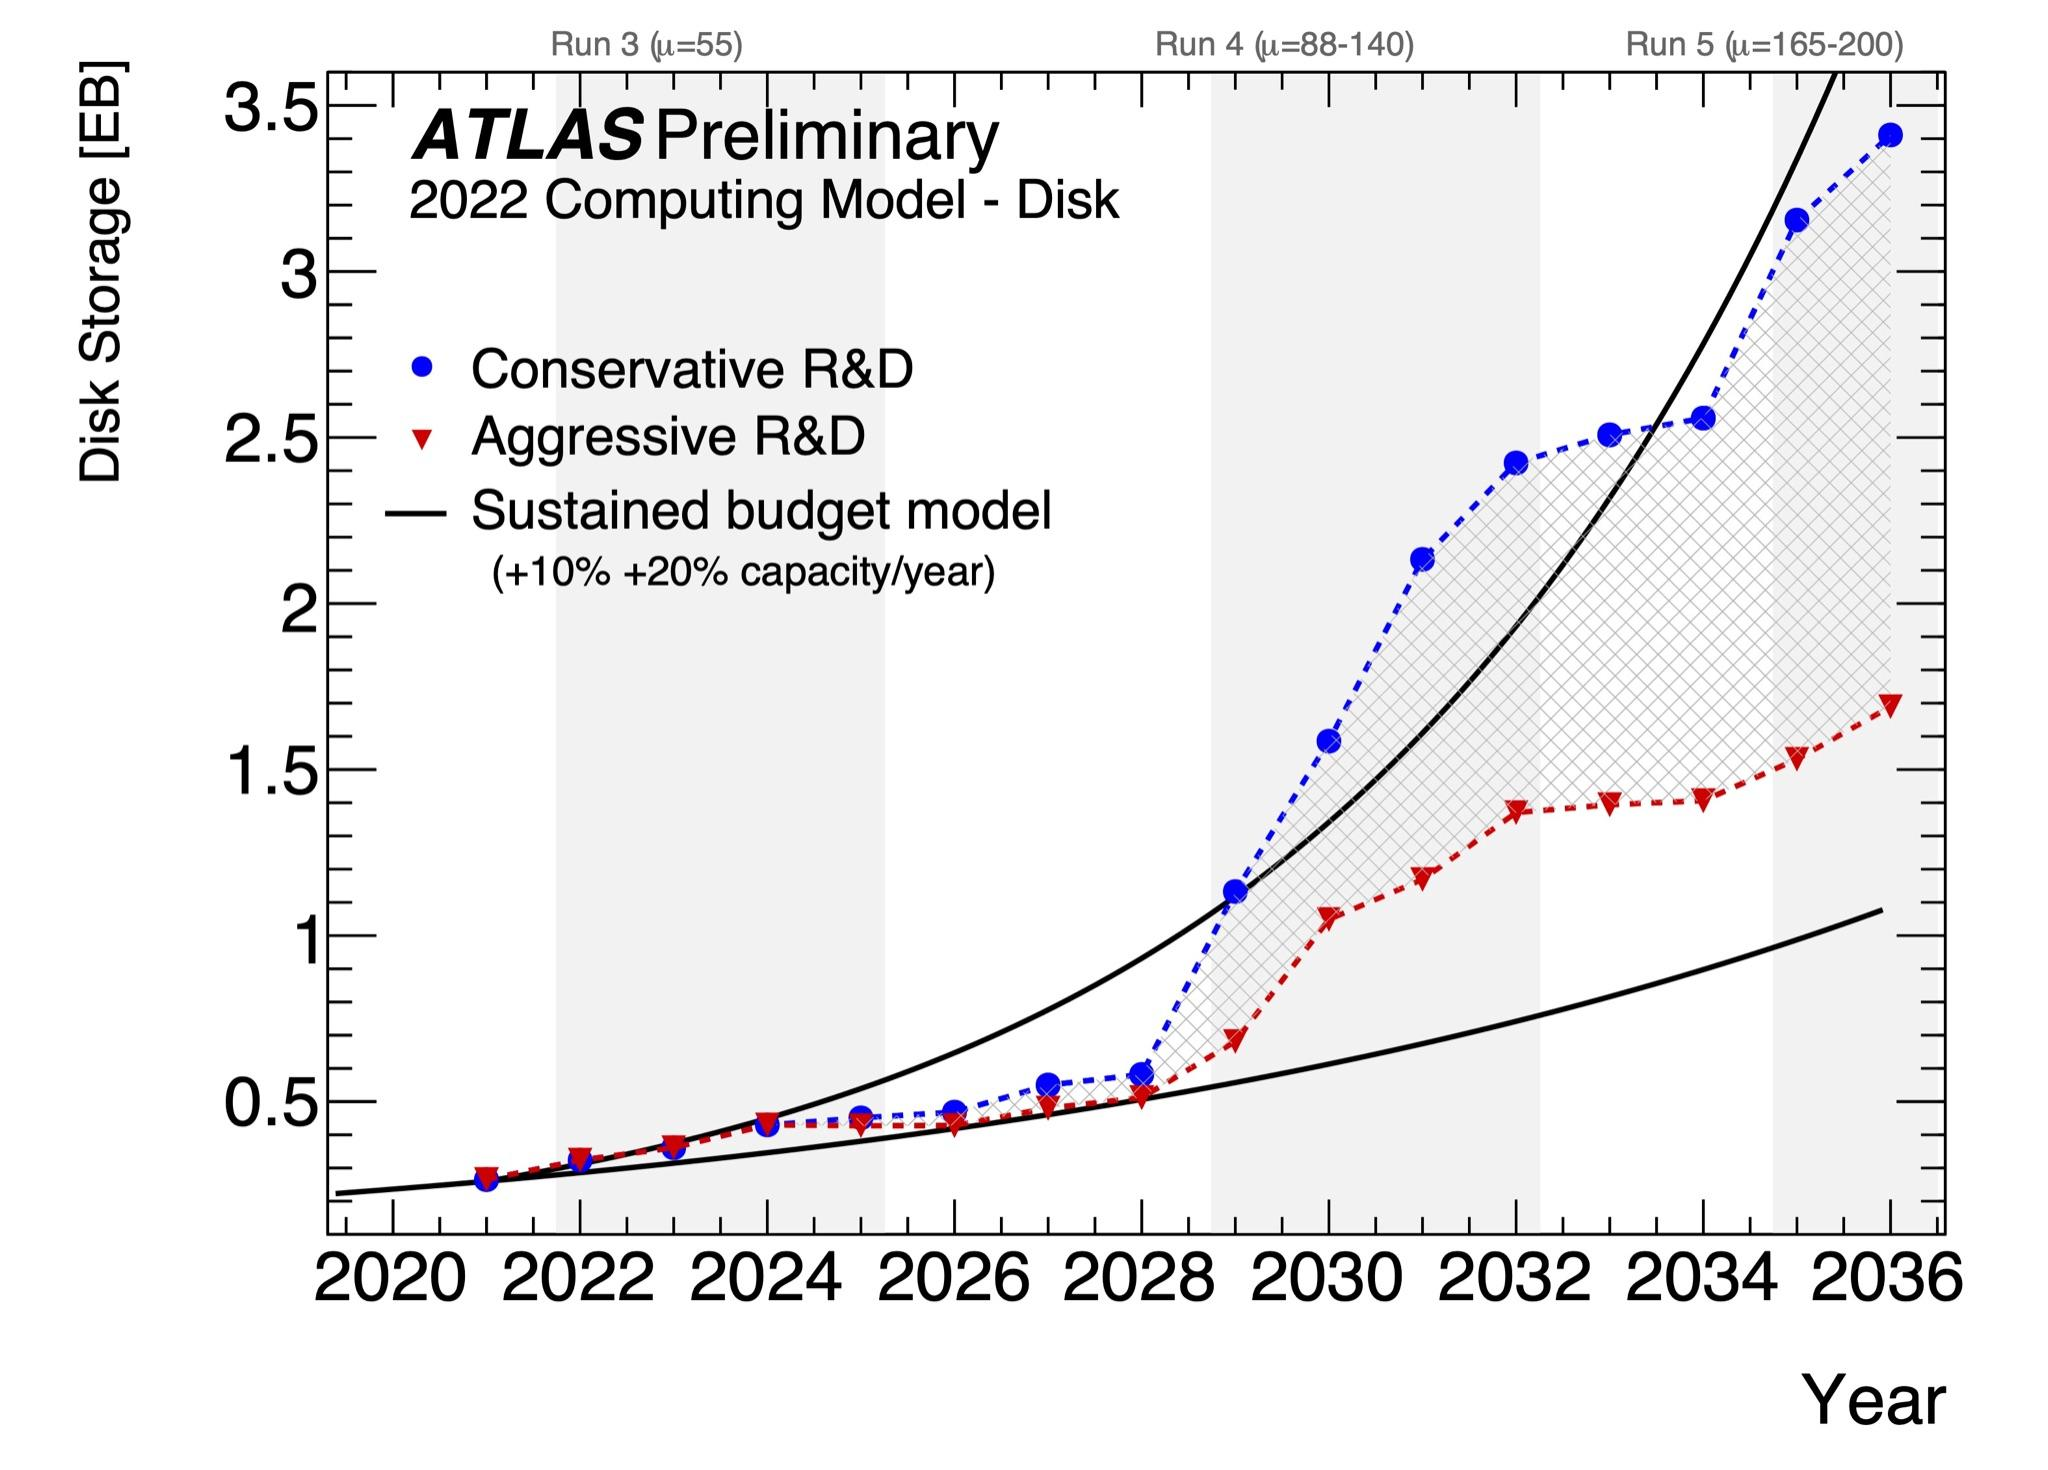
\includegraphics[width=0.8\textwidth]{atlas-disk-projection.png}
    \caption{Projected evolution of disk usage from 2020 until 2036, under the conservative (blue) and aggressive (red) R\&D scenarios.
The grey hatched shading between the red and blue lines illustrates the range of resources consumption if the aggressive scenario is only partially achieved.
The black lines indicate the impact of sustained year-on-year budget increases, and improvements in new hardware, that together amount to a capacity increase of 10\% (lower line) and 20\% (upper line).
The vertical shaded bands indicate periods during which ATLAS will be taking data.~\cite{CERN-LHCC-2022-005}}
    \label{fig:atlas-disk-projection}
\end{figure}

\section{Columnar Analysis Demonstrator}\label{sec:demonstrator}

One of the established research projects for columnar analysis is the development of an ATLAS columnar analysis demonstrator.
This demonstrator is inspired by the Institute for Research and Innovation in Software for High Energy Physics (IRIS-HEP)~\cite{S2I2HEPSP,CWPDOC} Analysis Grand Challenge~\cite{Held:2022sfw}, which leverages the ``PyHEP'' ecosystem of data science and analysis tools developed by IRIS-HEP and Scikit-HEP~\cite{Rodrigues:2020syo}.
These ecosystems of tools build upon and extend the broader Scientific Python ecosystem, with mature columnar analysis libraries, to provide functionality at each step of the columnar analysis pipeline: data query and access, data file I/O and columnar access, data transformation and histogramming, distributed analysis frameworks, statistical modelling and inference, and analysis reinterpretation.

The ATLAS Run 4 Analysis Model is built around the PHYSLITE common reduced data format~\cite{Schaarschmidt:2024vzr,SOFT-2022-02}.
PHYSLITE is a monolithic file format --- intended to support around 80\% of all physics analyses in Run 4 --- that contains already-calibrated physics objects for fast analysis, and allows for direct support without the need to create derived ROOT ntuples for analysis.
% The demonstrator uses ATLAS PHYSLITE open data~\cite{ATL-OREACH-PROC-2024-005,Marshall:2919097} --- released for research use for the first time in 2024 --- to ensure the accessibility and reproducibility of the technical demonstrator analysis.
The demonstrator uses ATLAS PHYSLITE open data~\cite{ATL-OREACH-PROC-2024-005} --- released for research use for the first time in 2024 --- to ensure the accessibility and reproducibility of the technical demonstrator analysis.
PHYSLITE has tight integration with ROOT features, to the extent that raw PHYSLITE is not easily loadable outside of ROOT in general.
Integrating PHYSLITE data access with the Python analysis ecosystem presents unique challenges, such as correctly reading unsplit objects with custom serialization and layout, e.g. \texttt{ElementLink}s~\cite{Hartmann:2021qzp} --- a smart pointer type for providing persistent references to a specific element in an object collection (``container'') --- and trigger data.
However, the Awkward Array~\cite{Awkward_Array_2018} library supports ``behaviors'' which allow for efficiently reinterpreting data structures on the fly, and can be used by Uproot~\cite{Uproot_2017} for I/O of custom serializations (e.g. PHYSLITE).
Through contributions by ATLAS members large amounts of PHYSLITE are now supported by both Uproot and Coffea~\cite{Coffea_2023,CMS:2020kpn} which allows for most workflows to proceed with small alterations~\cite{US_ATLAS_IRISHEP_trainging:2024}.
This allows for the demonstrator workflow to operate on most PHYSLITE files directly with Uproot, as seen in \Cref{fig:atlas-pipeline}.
For files in the PHYS ATLAS Run 3 Analysis Model data format~\cite{SOFT-2022-02}, FuncADL~\cite{funcadl_2024,Proffitt:2021wfh} and ServiceX~\cite{serviceX_2024,serviceX_client_2024,Galewsky:2020xig} can be used to create a distributed ROOT~\cite{Brun:1997pa} data transformation service to read the data and perform calibrations.
The result of the transform is an in-memory columnar representation equivalent to if the column had been read from PHYSLITE.
As PHYSLITE already contains all of the calibrated physics objects, it is preferable to use PHYSLITE whenever possible.

\begin{figure}
    \centering
    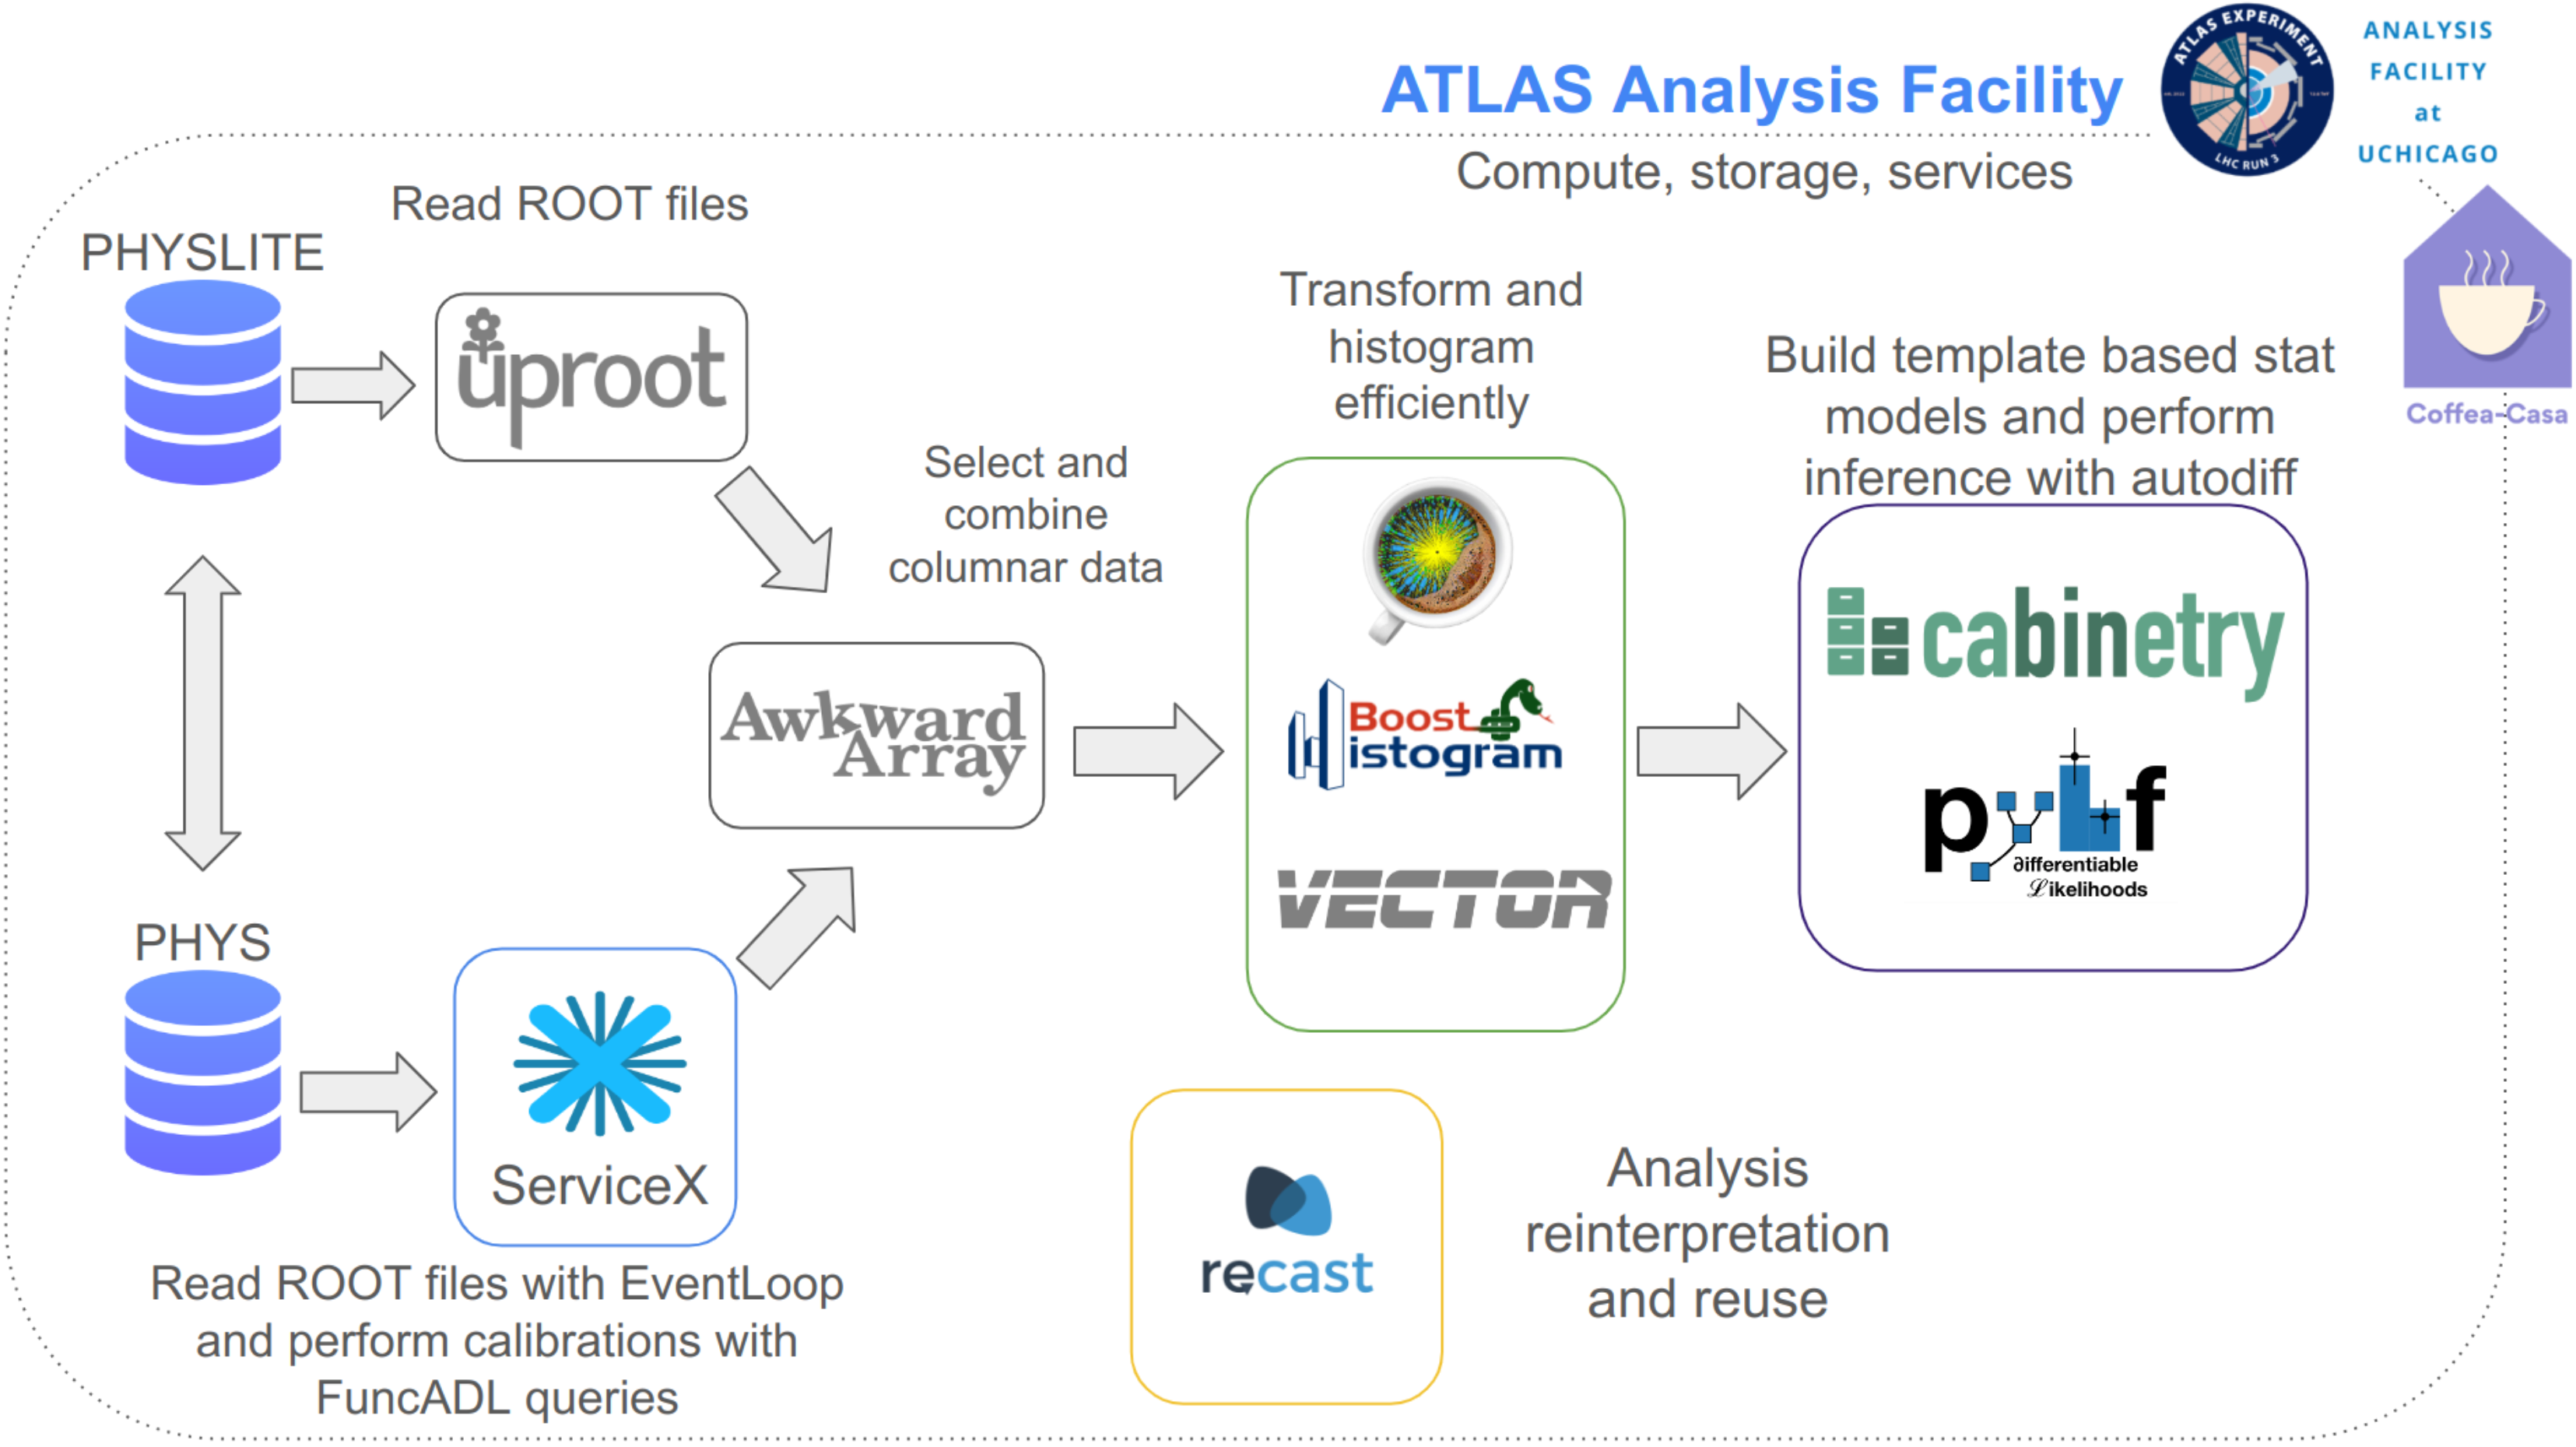
\includegraphics[width=\textwidth]{atlas-pipeline.png}
    \caption{Schematic outline of an ATLAS columnar analysis demonstrator able to operate on PHYS and PHYSLITE data formats using columnar analysis tools from the PyHEP ecosystem.
    The demonstrator is designed to be deployed and run at an ATLAS analysis facility, such as the University of Chicago Analysis Facility or a Coffea-casa deployment.}
    \label{fig:atlas-pipeline}
\end{figure}

\section{Challenges and Opportunities}\label{sec:challenges}

What becomes a challenge is when all branches of a PHYSLITE file need to be read including branches with custom objects and when systematics need to be handled.
As columnar analysis processes events in batches, this requires that ATLAS Combined Performance (CP) tools and algorithms must also be able to operate in batches.
The current model for CP tools is to operate on the ATLAS xAOD event data model (EDM) for all the calculations per event and then to write the systematics to disk for future access.
This process is I/O intensive, but has been computationally efficient for the current ATLAS analysis model.
The challenge for a fully columnar CP tool framework is to adapt to the on-the-fly computation of the columnar paradigm --- furthering the ``trade disk for compute'' strategy --- while still being performant enough to not be a bottleneck.

This refactoring process ongoing in the ATLAS Analysis Model Group (AMG) has also offered design improvement opportunities to create more Pythonic end-user APIs for the ATLAS CP tools.
As seen in~\Cref{fig:columnar_cp_tools_diagram}, creating Pythonic APIs for users allows for integration with the broader scientific Python ecosystem, but through efficient binding layers all data can be efficiently passed through to the \texttt{C++} CP tools for efficient computation, and then the results can be exposed to the users again.
By using \texttt{nanobind}~\cite{nanobind} --- next generation \texttt{C++}-to-Python bindings --- it becomes possible to have zero-copy operations to and from $n$-dimensional array libraries in Python, including those which support hardware accelerators like GPUs, and full design control of the high-level user API.
The API design ability is quite powerful, as it allows for unification of interfaces to CP tools without requiring individual CP tools to redesign their APIs.

\begin{figure}
    \centering
    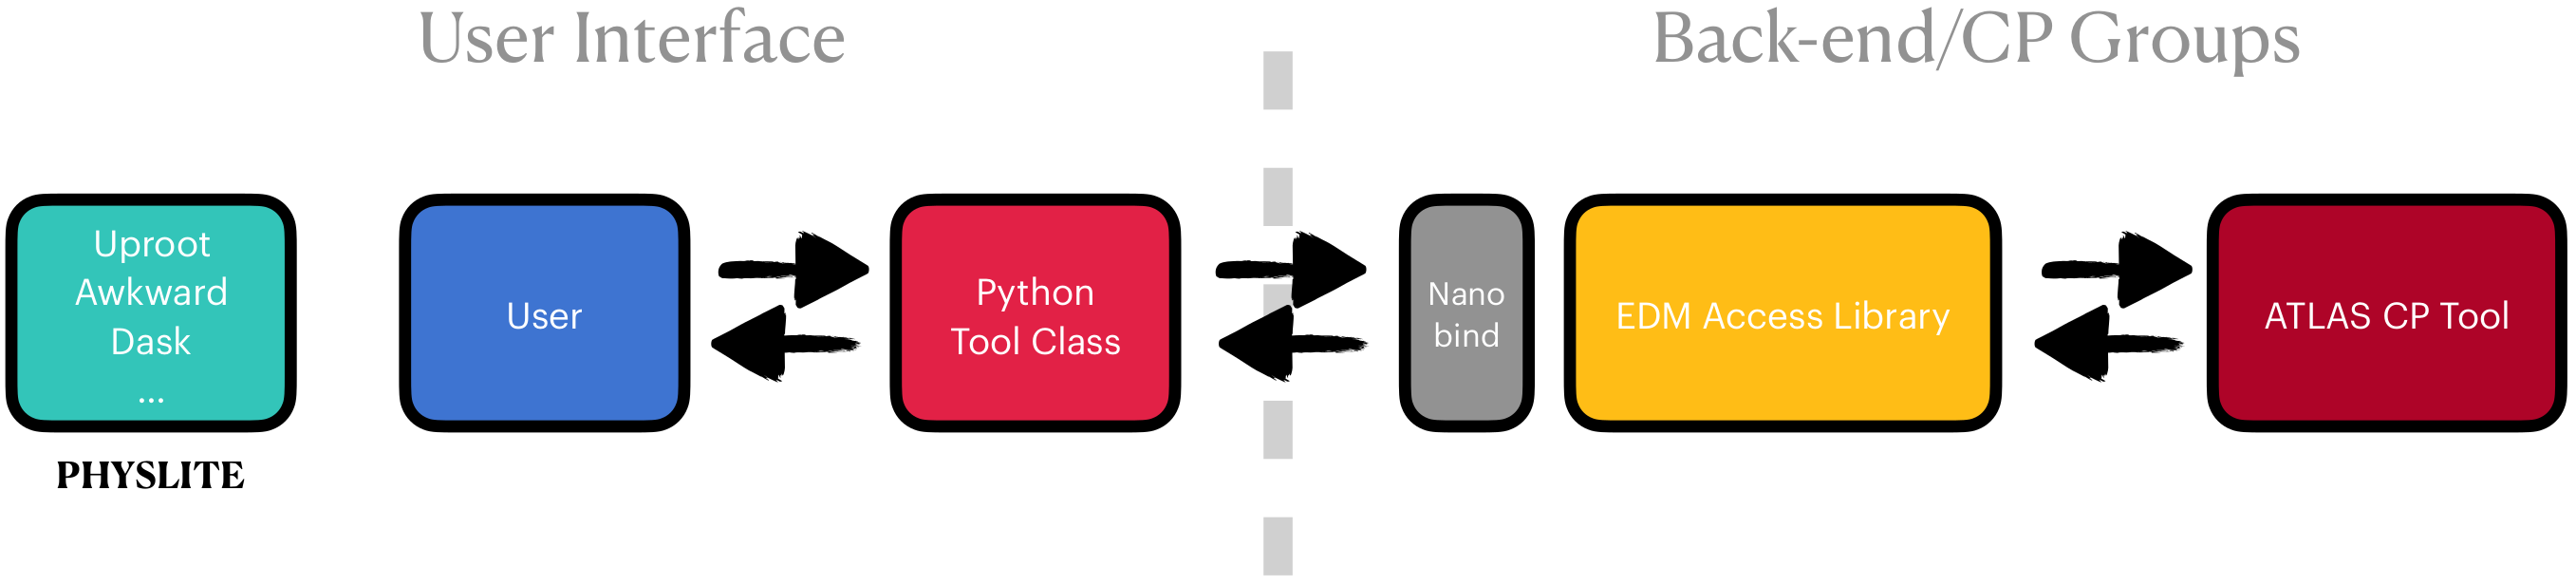
\includegraphics[width=\textwidth]{columnar_cp_tools_diagram.png}
    \caption{X~\cite{Vigl:ACAT_2024}.}
    \label{fig:columnar_cp_tools_diagram}
\end{figure}

\section{Columnar CP Prototypes}\label{sec:prototypes}

As a first (\texttt{v1}) prototype of this capability, a standalone columnar implementation of the ATLAS electron and photon (Egamma) CP tool with zero-copy \texttt{nanobind} Python bindings was created to compute on-the-fly systematics variations for the dilepton system mass in $e^{+}e^{-}$ final states.
Uproot was used to load ATLAS $Z\to \ell\ell$ simulation PHYSLITE files into Awkward arrays, and the $e^{+}e^{-}$ event selections were applied with Coffea.
The columnar Egamma tool was initialized through the Pythonic interface, \texttt{atlascp.EgammaTools}, and then passed Awkward arrays of electrons to compute on-the-fly systematic variations of the electron reconstruction efficiency scale factors and energy correction resolution and scale, from which the corrected dilepton mass was computed.
The computations were additionally scaled out with \texttt{dask-awkward}~\cite{dask_awkward_2024} on the University of Chicago ATLAS Analysis Facility to minimize the compute wall time, with the gathered results visualized in~\Cref{fig:Zee_mc_systematics}.

This preliminary research was required as there was no ```zero action'' option to determine the viability of the proposed design \textit{a priori}.
The \texttt{v1} prototype established the foundations of what was possible with new tooling and that Pythonic interfaces to CP tools could be written without large amounts of work or deep knowledge of underlying CP tool design.
This showed a promising direction, but additional work is needed to achieve the necessary performance, integration, and support required for use.

A \texttt{v2} ``Columnar Athena'' prototype~\cite{columnar_athena} has been started to expand on the scope of the \texttt{v1} prototype.
This moves the development of the columnar tools and interfaces from individual standalone examples into a unified system under the ATLAS Athena framework~\cite{ATLAS_Athena} and migrates the ATLAS CP tools to a columnar backend without breaking the existing workflows using the EDM models.
It additionally adds infrastructure support for development of columnar analysis tools by adding \texttt{nanobind} to the ATLAS Externals tooling distributed as part of the ATLAS Athena Analysis Releases.
While currently under active development, the \texttt{v2} prototype will allow for full scale integration and performance tests of the columnar CP tools and interfaces.

\begin{figure}
    \centering
    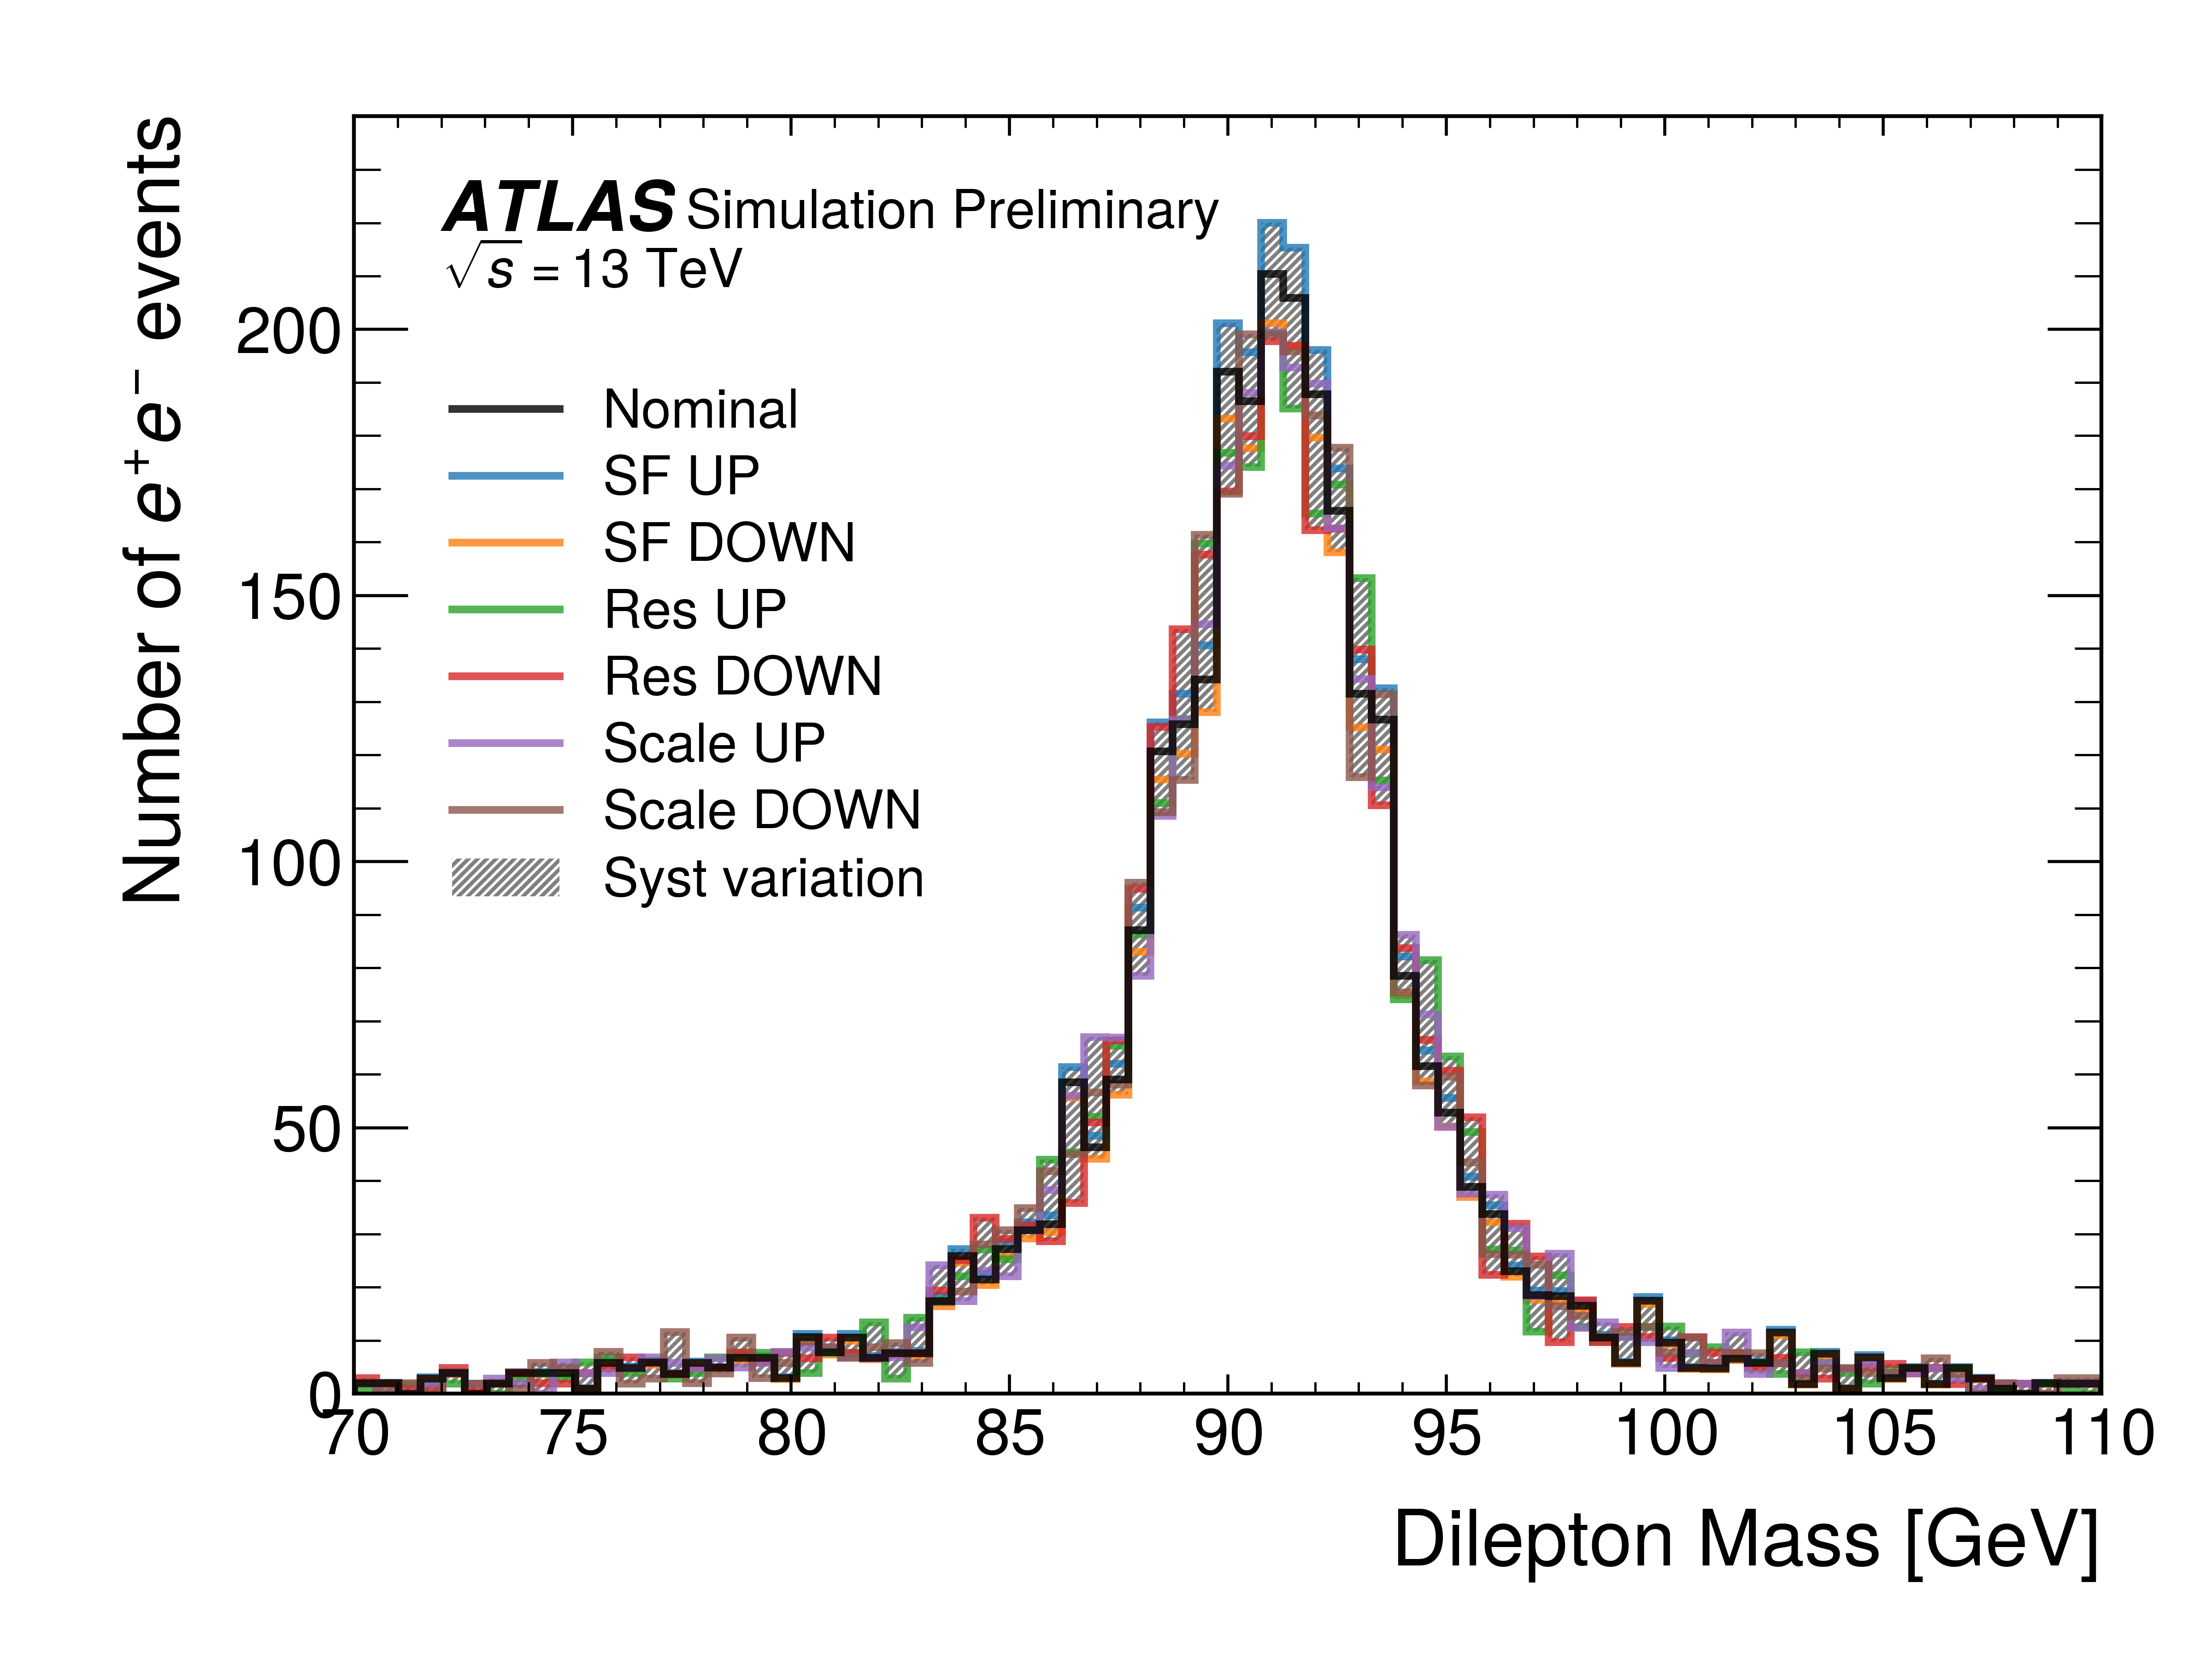
\includegraphics[width=0.7\textwidth]{Zee_mc_systematics.png}
    \caption{Histograms of the dilepton mass of selected $Z\to e^{+}e^{-}$ events in ATLAS simulation under on-the-fly systematic variations of the electron reconstruction efficiency scale factor (SF) --- the product of the reconstruction, identification, and isolation scale factors --- and energy correction resolution (Res) and scale (Scale)~\cite{Vigl:ACAT_2024}.}
    \label{fig:Zee_mc_systematics}
\end{figure}

\section{Preliminary Performance Tests and Future Decisions and Work}\label{sec:conclusions}

During the ongoing refactor for the \texttt{v2} prototype, preliminary integrated benchmarks have been created to measure the time spent in each tool per event (excluding I/O) in comparison with the xAOD model.
While direct one-to-one comparisons are not possible given the inherent differences in data processing, the tests have been designed to be as close as possible.
The benchmarks compare the same version of each cP tool, only use the \texttt{C++} code (no Python is involved so as to isolate the \texttt{C++} performance), and the time for the xAOD model includes the event store access overhead (which is per-event for the xAOD model and per-batch for the columnar model).
The time for I/O and connecting columns is also not included in the performance comparisons, as this has not been optimized in the current tests and will not provide useful information, and so are removed from the benchmark.
The benchmarks show substantial speedups for the migrated tools with the columnar implementations ranging from being \emph{2-4x faster} than the xAOD interface.
The specific reasons for the speedups are currently being investigated fully, but preliminary checks show a relation with EDM access (columnar tools need to access the EDM once per event batch).

ATLAS CP tools were created 10-15 years ago to run in an analysis framework.
Battle tested, extremely well understood, excellent physics performance, strong desire to be maintained.
Rewrite cost is currently too high across collaboration to move to \texttt{correctionlib} paradigm.
Columnar cracks open ``black box'' implementations of tools for the new analysis model.
Legacy code decisions highlight columnar prototype design decisions and opportunities during tool migration.
Raises the question: ``What would it take to get to \texttt{python -m pip install atlascp}?''
Columnar prototype explores these possibilities.
Steps beyond: Modularization to level that allows packaging with \texttt{scikit-build-core}.



\section{Acknowledgements}\label{sec:acknowledgements}

Matthew Feickert, Alexander Held, and Gordon Watts are supported by the U.S. National Science Foundation (NSF) under Cooperative Agreement OAC-1836650 and PHY-2323298 (IRIS-HEP).
Lukas Heinrich and Evangelos Kourlitis are supported by the Excellence Cluster ORIGINS, which is funded by the Deutsche Forschungsgemeinschaft (DFG, German Research Foundation) under Germany's Excellence Strategy - EXC-2094-390783311 and by the German Federal Ministry of Education and Research Project 05H2021 (ErUM-FSP T02) - ``Run 3 von ATLAS am LHC: Analysis Infrastructure for the ATLAS Detektor at the LHC''.


% Don't use \bibliographystyle
% the style is already called in woc.bst, so ensure it is in the top level directory
\bibliography{bib/ref}

\end{document}

<div id='footer'><table width='100%'><tr><td class='right'><a href='http://fusioninventory.org/'><span class='copyright'>FusionInventory 9.1+1.0 | copyleft <img src='/glpi/plugins/fusioninventory/pics/copyleft.png'/>  2010-2016 by FusionInventory Team</span></a></td></tr></table></div>
